% Options for packages loaded elsewhere
\PassOptionsToPackage{unicode}{hyperref}
\PassOptionsToPackage{hyphens}{url}
%
\documentclass[
  11pt,
  ignorenonframetext,
]{beamer}
\usepackage{pgfpages}
\setbeamertemplate{caption}[numbered]
\setbeamertemplate{caption label separator}{: }
\setbeamercolor{caption name}{fg=normal text.fg}
\beamertemplatenavigationsymbolsempty
% Prevent slide breaks in the middle of a paragraph
\widowpenalties 1 10000
\raggedbottom
\setbeamertemplate{part page}{
  \centering
  \begin{beamercolorbox}[sep=16pt,center]{part title}
    \usebeamerfont{part title}\insertpart\par
  \end{beamercolorbox}
}
\setbeamertemplate{section page}{
  \centering
  \begin{beamercolorbox}[sep=12pt,center]{part title}
    \usebeamerfont{section title}\insertsection\par
  \end{beamercolorbox}
}
\setbeamertemplate{subsection page}{
  \centering
  \begin{beamercolorbox}[sep=8pt,center]{part title}
    \usebeamerfont{subsection title}\insertsubsection\par
  \end{beamercolorbox}
}
\AtBeginPart{
  \frame{\partpage}
}
\AtBeginSection{
  \ifbibliography
  \else
    \frame{\sectionpage}
  \fi
}
\AtBeginSubsection{
  \frame{\subsectionpage}
}
\usepackage{amsmath,amssymb}
\usepackage{lmodern}
\usepackage{iftex}
\ifPDFTeX
  \usepackage[T1]{fontenc}
  \usepackage[utf8]{inputenc}
  \usepackage{textcomp} % provide euro and other symbols
\else % if luatex or xetex
  \usepackage{unicode-math}
  \defaultfontfeatures{Scale=MatchLowercase}
  \defaultfontfeatures[\rmfamily]{Ligatures=TeX,Scale=1}
\fi
\usetheme[]{metropolis}
% Use upquote if available, for straight quotes in verbatim environments
\IfFileExists{upquote.sty}{\usepackage{upquote}}{}
\IfFileExists{microtype.sty}{% use microtype if available
  \usepackage[]{microtype}
  \UseMicrotypeSet[protrusion]{basicmath} % disable protrusion for tt fonts
}{}
\makeatletter
\@ifundefined{KOMAClassName}{% if non-KOMA class
  \IfFileExists{parskip.sty}{%
    \usepackage{parskip}
  }{% else
    \setlength{\parindent}{0pt}
    \setlength{\parskip}{6pt plus 2pt minus 1pt}}
}{% if KOMA class
  \KOMAoptions{parskip=half}}
\makeatother
\usepackage{xcolor}
\newif\ifbibliography
\usepackage{graphicx}
\makeatletter
\def\maxwidth{\ifdim\Gin@nat@width>\linewidth\linewidth\else\Gin@nat@width\fi}
\def\maxheight{\ifdim\Gin@nat@height>\textheight\textheight\else\Gin@nat@height\fi}
\makeatother
% Scale images if necessary, so that they will not overflow the page
% margins by default, and it is still possible to overwrite the defaults
% using explicit options in \includegraphics[width, height, ...]{}
\setkeys{Gin}{width=\maxwidth,height=\maxheight,keepaspectratio}
% Set default figure placement to htbp
\makeatletter
\def\fps@figure{htbp}
\makeatother
\setlength{\emergencystretch}{3em} % prevent overfull lines
\providecommand{\tightlist}{%
  \setlength{\itemsep}{0pt}\setlength{\parskip}{0pt}}
\setcounter{secnumdepth}{-\maxdimen} % remove section numbering
\ifLuaTeX
  \usepackage{selnolig}  % disable illegal ligatures
\fi
\IfFileExists{bookmark.sty}{\usepackage{bookmark}}{\usepackage{hyperref}}
\IfFileExists{xurl.sty}{\usepackage{xurl}}{} % add URL line breaks if available
\urlstyle{same} % disable monospaced font for URLs
\hypersetup{
  pdftitle={Conceptos básicos de estadística},
  pdfauthor={Gerardo Martín},
  hidelinks,
  pdfcreator={LaTeX via pandoc}}

\title{Conceptos básicos de estadística}
\subtitle{Poblaciones y muestras}
\author{Gerardo Martín}
\date{2022-06-29}

\begin{document}
\frame{\titlepage}

\hypertarget{poblaciuxf3n}{%
\section{Población}\label{poblaciuxf3n}}

\begin{frame}{¿Qué entienden por población?}
\protect\hypertarget{quuxe9-entienden-por-poblaciuxf3n}{}
\begin{itemize}
\tightlist
\item
  ``Población de Mérida'' vs.~``Población de estudio''
\end{itemize}
\end{frame}

\begin{frame}{¿Qué entienden por población?}
\protect\hypertarget{quuxe9-entienden-por-poblaciuxf3n-1}{}
\begin{itemize}
\tightlist
\item
  \emph{Población} - Grupo que se va a estudiar
\item
  \emph{Muestra} - Individuos de la población de estudio
\item
  \emph{Individuos} - Personas, animales u objetos que forman la muestra
\end{itemize}
\end{frame}

\begin{frame}{De poblaciones a individuos}
\protect\hypertarget{de-poblaciones-a-individuos}{}
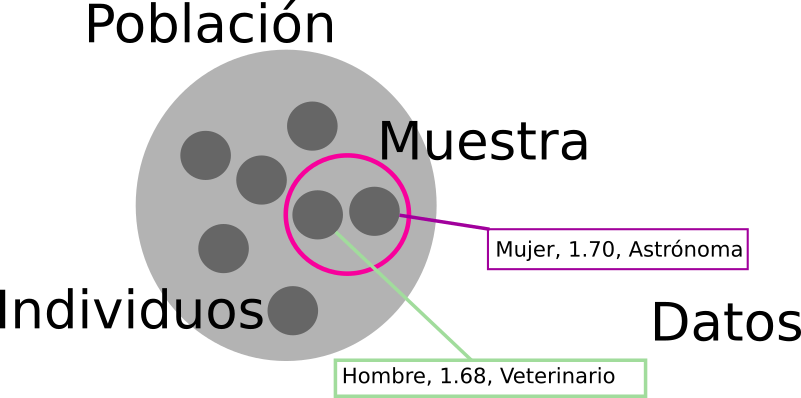
\includegraphics{Figuras-Intro/Poblacion-indiv.png}
\end{frame}

\begin{frame}{Importancia}
\protect\hypertarget{importancia}{}
\begin{center}
\includegraphics[width=8.33in]{Figuras-Intro/mundo} \end{center}
\end{frame}

\begin{frame}{Importancia}
\protect\hypertarget{importancia-1}{}
\begin{itemize}
\item
  No se puede estudiar todo

  \begin{itemize}
  \tightlist
  \item
    Dificultades logísticas
  \item
    Dificultades económicas
  \end{itemize}
\item
  Fenómenos de relevancia regional
\item
  Diferentes escalas
\end{itemize}
\end{frame}

\begin{frame}{Ejemplos}
\protect\hypertarget{ejemplos}{}
\begin{itemize}
\tightlist
\item
  \textbf{Población}: Ciudad Caucel
\item
  \textbf{Muestra}: 10 familias de cada colonia
\item
  \textbf{Individuo}: Integrantes de la familia
\end{itemize}
\end{frame}

\begin{frame}{Ejemplos}
\protect\hypertarget{ejemplos-1}{}
\begin{itemize}
\tightlist
\item
  \textbf{Población}: Industria pecuaria de Hunucmá
\item
  \textbf{Muestra}: Granjas porcícolas \textless{} 1 km de cenotes
\item
  \textbf{Individuo}: 1 L de desecho de lagunas de oxidación
\end{itemize}
\end{frame}

\begin{frame}{Criterios para seleccionar población, muestra e individuo}
\protect\hypertarget{criterios-para-seleccionar-poblaciuxf3n-muestra-e-individuo}{}
\begin{itemize}
\item
  Objetivo del estudio

  \begin{itemize}
  \tightlist
  \item
    ¿Qué se quiere demostrar?
  \item
    Pregunta científica concreta
  \item
    Análisis estadísticos a realizar
  \item
    Hipótesis que a probar
  \end{itemize}
\item
  Datos necesarios

  \begin{itemize}
  \tightlist
  \item
    Mediciones de l\_s individu\_s
  \item
    Cuánt\_s individu\_s
  \item
    Características de l\_s individu\_s
  \end{itemize}
\end{itemize}
\end{frame}

\hypertarget{ejemplos-2}{%
\section{Ejemplos}\label{ejemplos-2}}

\begin{frame}{¿Cómo afecta la ganadería la calidad del agua?}
\protect\hypertarget{cuxf3mo-afecta-la-ganaderuxeda-la-calidad-del-agua}{}
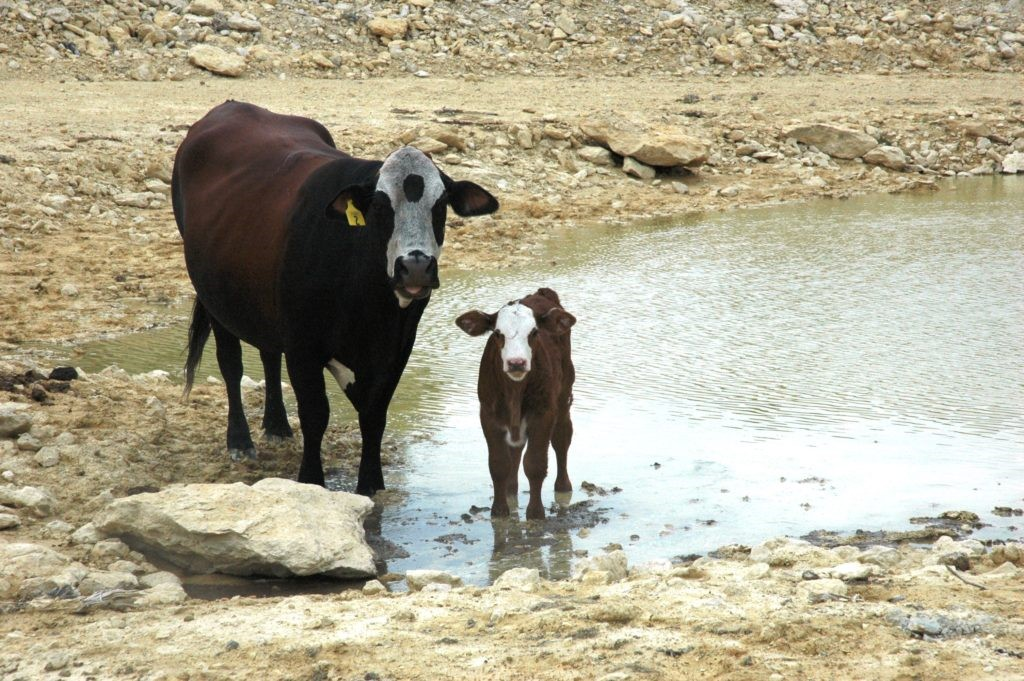
\includegraphics{Figuras-Intro/Cattle-water.jpg}
\end{frame}

\begin{frame}{¿Dónde colectarían el agua?}
\protect\hypertarget{duxf3nde-colectaruxedan-el-agua}{}
\begin{enumerate}
\tightlist
\item
  Donde hay ganado
\item
  Donde no hay ganado
\item
  Dentro del rancho
\item
  Fuera del rancho
\item
  Río abajo o arriba del rancho
\end{enumerate}
\end{frame}

\begin{frame}{Propuesta}
\protect\hypertarget{propuesta}{}
\begin{enumerate}
\tightlist
\item
  Objetivo
\item
  Hipótesis
\item
  Pregunta específica
\item
  Determinar qué se medirá
\item
  Determinar cómo se analizará
\item
  Determinar cuántos datos
\item
  Determinar población
\item
  Seleccionar muestra
\item
  Muestrear
\item
  Analizar
\end{enumerate}
\end{frame}

\end{document}
